\section{Neural Ordinary Differential Equations}
\label{sec:literature-review-neural-ordinary-differential-equations}

When modeling dynamical systems, it is generally challenging to create a model by hand because real-world data are often hard to interpret or are sampled at an irregular interval.
Using \glspl{NeuralODE}, the system's dynamics can be learned through data-driven approaches without having explicitly specified \glspl{ODE} or \glspl{PDE}.
\glspl{NeuralODE} can also be used to replace a stack of residual blocks because they perform the same functionality while reducing the memory cost of training the model.
\citeauthor{chenNeuralOrdinaryDifferential2019} made an observation that models such as residual networks (see \autoref{fig:residual-network-skip-connection}), \gls{RNN} decoders, or normalizing flows build complex transformations by composing a sequence of modifications to a hidden state \cite{chenNeuralOrdinaryDifferential2019}
\begin{equation*}
    h_{t+1} = h_t + f(h_t, \theta_t)
\end{equation*}
where $t \in \{0 \cdots T\}$ and $h_t \in \mathbb{R}^D$.
These iterative updates can be seen as an Euler discretization of a continuous transformation.
In \gls{NeuralODE}, the continuous dynamics of hidden units are parameterized using an \gls{ODE} specified by an \gls{ANN}
\begin{equation*}
    \frac{dh(t)}{dt} = f(h(t), t, \theta).
\end{equation*}
That is starting from the input layer $h(0)$, the output layer $h(T)$ can be defined as the solution to the \gls{ODE} initial value problem at time step $T$.
Typical \glspl{ANN} create a mapping from the inputs to the outputs, whereas \glspl{NeuralODE} define the dynamics that can turn the inputs into the outputs.
There are several benefits when doing this, such as:
\begin{itemize}
    \item \textbf{Memory efficiency}
    Computing the gradients of the loss function with respect to all the inputs of the \gls{ODE} solver does not require back-propagation.
    Thus, intermediate values of the forward pass do not need to be stored.
    This allows for training with constant memory cost.
    \item \textbf{Adaptive computation}
    Modern \gls{ODE} solver guarantees the growth of approximation error.
    They keep track of errors and adapt the evaluation strategy to provide the requested level of accuracy.
    The cost of evaluating the model can scale with the problem's complexity.
    \item \textbf{Scalable and invertible normalizing flows}
    Continuous transformations allow the change of variables formula to become easier to compute.
    \item \textbf{Continuous time-series models}
    Continuously defined dynamics can incorporate data that arrive at arbitrary times.
    Network models such as \glspl{RNN} require the discretization of observation and emission intervals
\end{itemize}

\begin{figure}
    \centering
    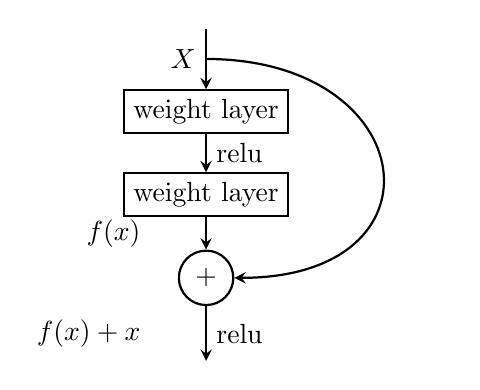
\begin{tikzpicture}[->, >=stealth, node distance = 3em, thick]
        \tikzset{
            block/.style  = {draw, thick, rectangle},
            arith/.style  = {draw, thick, circle},
            input/.style  = {coordinate},
            output/.style = {coordinate}
        }
        \node[input] (IN) {};
        \node[block, below of = IN] (W1) {weight layer};
        \node[block, below of = W1] (W2) {weight layer};
        \node[arith, below of = W2] (ADD) {+};
        \node[output, below of = ADD] (OUT) {+};

        \draw[->] (IN) to node[left, name = X]{$X$} (W1);
        \draw[->] (X) to [out = 0, in = 0, looseness = 2.5] (ADD);
        \draw[->] (W1) to node[right]{relu} (W2);
        \draw[->] (W2) to node[xshift = -2em, left]{$f(x)$} (ADD);
        \draw[->] (ADD) to node[xshift = -2em, left]{$f(x) + x$} node[right]{relu} (OUT);
    \end{tikzpicture}
    \caption{Example of a skip connection in residual network}
    \label{fig:residual-network-skip-connection}
\end{figure}

For a \gls{NeuralODE} to be trainable with gradient descent, we must have a way to compute the gradients of the loss with respect to the parameters of the \gls{NeuralODE}.
The regular method for taking the loss gradients in \glspl{ANN} (back-propagation) can not be applied for \glspl{NeuralODE} because it incurs high memory cost and introduces additional numerical errors.
Hence, the authors of the method use \textit{adjoint sensitivity analysis} to compute the gradients.
The gradients are computed by solving a second, augmented \gls{ODE} backward in time.
This method applies to all \gls{ODE} solvers.
The approach scales linearly with the problem size, and the numerical error can be controlled explicitly.
\autoref{alg:neural-ode-reverse-mode-diff} shows the overall steps that need to be taken to compute the derivatives.
We consider the loss function $L$, which takes the result of an \gls{ODE} solver
\begin{equation*}
    L(z(t_1)) = L\left(z(t_0) + \int_{t_0}^{t_1}{f(z(t), t, \theta)dt}\right) = L(ODESolve(z(t_0), f, t_0, t_1, \theta)).
\end{equation*}
First, we consider the gradient of the loss with respect to the hidden state $z(t)$, called the adjoint $a(t) = \partial L / \partial z(t)$.
The dynamics of the adjoint are then given by another \gls{ODE}
\begin{equation*}
    \frac{da(t)}{dt} = -a(t)^T\frac{\partial f(z(t), t, \theta)}{\partial z}.
\end{equation*}
The gradient of the loss with respect to the hidden state at the initial time step can be calculated by integrating the adjoint dynamics backward in time starting from the value $\partial L / \partial z(t_1)$
\begin{equation}
    \frac{dL}{dz(t_0)} = \frac{\partial L}{\partial z(t_1)} + \int_{t_1}^{t_0}{-a(t)^T\frac{\partial f(z(t), t, \theta)}{\partial z}} dt.
    \label{eq:neural-ode-loss-wrt-initial-hidden-state}
\end{equation}
Computing $dL/dz(t_0)$ requires the hidden state $z(t)$ at each evaluated time step which is calculated by integrating the dynamics of our system backward in time starting from the value $z(t_1)$
\begin{equation}
    z(t) = z(t_1) + \int_{t_1}^{t}{f(z(t), t, \theta)dt}.
    \label{eq:neural-ode-hidden-state-backward-integral}
\end{equation}
Finally, we can calculate the gradients of the loss function with respect to the parameters $\theta$ using
\begin{equation}
    \frac{dL}{d\theta} = \int_{t_1}^{t_0}{-a(t)^T\frac{\partial f(z(t), t, \theta)}{\partial \theta}} dt.
    \label{eq:neural-ode-loss-wrt-parameters}
\end{equation}
The vector-Jacobian products $a(t)^T\frac{\partial f}{\partial z}$ and $a(t)^T\frac{\partial f}{\partial \theta}$ from \autoref{eq:neural-ode-loss-wrt-initial-hidden-state} and \autoref{eq:neural-ode-loss-wrt-parameters} can be computed efficiently with automatic differentiation.
The integrals in \autoref{eq:neural-ode-loss-wrt-initial-hidden-state}, \autoref{eq:neural-ode-hidden-state-backward-integral}, and \autoref{eq:neural-ode-loss-wrt-parameters} can be computed in a single call to an \gls{ODE} solver.

\begin{algorithm}
    \caption{Reverse-mode derivative of an ODE initial value problem (taken from \cite{chenNeuralOrdinaryDifferential2019})}
    \label{alg:neural-ode-reverse-mode-diff}
    \begin{algorithmic}
        \Function{ODEDerivative}{$\theta, t_0, t_1, z(t_1), \frac{\partial L}{\partial z(t_1)}$}
            \State $s_0 \gets \left[z(t_1), \frac{\partial L}{\partial z(t_1)}, 0_{|\theta|}\right]$
            \Comment{Define initial augmented state}
            \Function{AugDynamics}{$\left[z(t), a(t), \cdot\right], t, \theta$}
            \Comment{Define dynamics on augmented state}
                \State \Return $\left[f(z(t), t, \theta), -a(t)^T\frac{\partial f}{\partial z}, -a(t)^T\frac{\partial f}{\partial \theta}\right]$
                \Comment{Compute vector-Jacobian products}
            \EndFunction
            \State $\left[z(t_0), \frac{\partial L}{\partial z(t_0)}, \frac{\partial L}{\partial \theta}\right] \gets \Call{ODESolve}{s_0, \textproc{AugDynamics}, t_1, t_0, \theta}$
            \Comment{Solve ODE backward}
            \State \Return $\left[\frac{\partial L}{\partial z(t_0)}, \frac{\partial L}{\partial \theta}\right]$
            \Comment{Return the gradients}
        \EndFunction
    \end{algorithmic}
\end{algorithm}